\documentclass[titlepage=firstcover, captions=tableheading]{scrartcl}
\usepackage{microtype}
\usepackage{amsmath}
\usepackage{polyglossia}
\usepackage{graphicx}
\usepackage{booktabs}
\usepackage{siunitx}
\usepackage{hyperref}
\usepackage{caption}
\usepackage{float}
\setdefaultlanguage{german}

\begin{document}
    
\section{Auswertung}

\subsection{Geometrische Abmessungen}

In der Folgenden Tabelle werden die geometrischen Abmessungen der verwendeten Kupferproben dargestellt.
Dabei gibt es für die Kupferfolie eine Höhe (H), eine Breite(b) und eine Dicke (d) sowie einen Durchmesser (D) und eine Länge (L) des Kupferdrahtes.

\begin{center}
    \captionof{table}{Geometrische Abmessungen in cm}
    \begin{tabular}{lllll}
        \toprule
        H & b & d & D & L \\
        \midrule 
        0.026 & 0.028 & 0.00043 & 0.000263 & 173 \\
        \bottomrule
    \end{tabular}
\end{center}

\subsection{Widerstand}

Der Widerstand wurde bei der Durchführung des Versuchs direkt mit einem Multimeter gemessen.
Dafür musste lediglich das Messgerät an den Kupferdraht angeschlossen werden und mit den richtigen Einstellungen zeigt es einen Widerstand von 9.7 \Omega \; an.

\subsection{Hall Effekt}

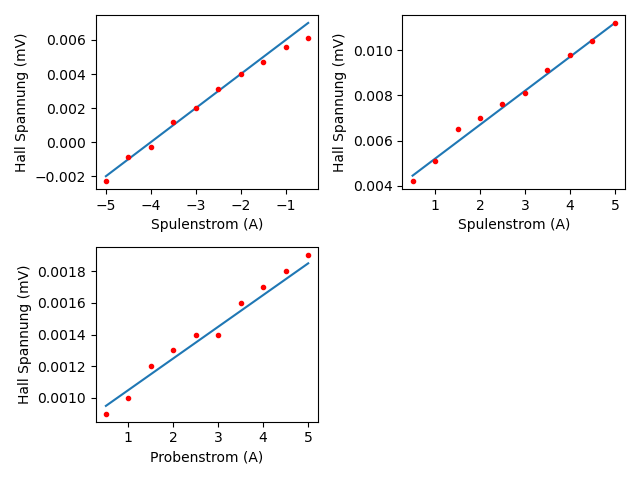
\includegraphics{plothall.png}

In den Koordinatensystemen sind die gemessenen Hall-Spannungen aufgetragen.
Zu den Geaphen ist zu sagen, dass auf der x-Achse entweder der Spulenstrom oder der Probenstrom abgebildet wird.
Die jewils andere Stromstärke wird konstant bei 5A gehalten.

\subsection{Ladungsträger pro Volumen n}

n lässt sich mit der Formel ? brechnen.
Um mit dieser Formel zu rechnen ist es notwendig, die Magnetfeldstärke in abhängigkeit der Stromstärke zu kennen.
Dieser Zusammenhang ist durch die Messwerte gegeben.
Ebenso sind die gemessenen Hall-Spannungen für diese Rechnung notwendig.

Daraus lässt sich die Ladungsdichte bestimmen.

\begin{minipage}{\linewidth}
    \centering
\captionof{table}{Ladungsdichte der Kupferprobe}
\begin{tabular}{ll}
    \toprule
    Stromstärke (A) & Magnetfeldstärke (T) \\
    \midrule
    0.5 &  
    1   &     
    1.5 &  
    2   &  
    2.5 &  
    3   &  
    3.5 &  
    4   &  
    4.5 &  
    5   &      \\
    \bottomrule
    
\end{tabular}
\end{minipage}

\end{document}